%%This is a very basic article template.
%%There is just one section and two subsections.
\documentclass{article}
%\documentclass[a4paper,12pt,twoside,brazil]{article}

\usepackage[top=25mm,bottom=20mm,left=20mm,right=15mm]{geometry} %coloca o tamanho das margens
\usepackage[T1]{fontenc}        % pacote para conj. de caracteres correto
\usepackage[utf8]{inputenc}     % pacote para acentuação
\usepackage[brazil]{babel}

\begin{document}

\title{RELATÓRIO CIENTÍFICO}

\section{Relatório Científico}

\subsection{Subtitle}

Plain text.

\subsection{Another subtitle}

More plain text.






Relatório Cinetífico

Processo #2012/04555-4

Resumo

- resumo do plano inicial e das etapas ja descritas em relatorios anteriores


a primeira etapa do projeto consiste na obtenção de dados tridimensionais a
partir de uma câmera estéreo. Está sendo utlilizado como equipamentos duas
abordagens. A primeira utilizando uma camera estéreo Bumblebee 2 que já possui
duas lentes dispostas de forma fixa permitindo um campo de visão restrito. A
outra abordagem é o uso de duas (ou três) cameras simples do tipo Flea podendo
serem dispostas com certa liberdade para formar o conjunto estéreo e assim ter
um campo de visão ajustado de acordo com a necessidade. Ambas abordagens
requerem uma calibração das lentes e do conjunto estéreo, sendo a segunda
abordagem mais sucetivel a problemas de descalibração por trepidações e
desregulagem dos seus posicionamentos provocada por vibrações.





- Resumo do que foi realizado no período a que se refere o relatório

) foram concluidas as disciplinas do mestrado contabilizando 58 créditos (sendo
48 obrigatórios) todas com conceito de aprovação A. 
) aprovação no exame de proficiência em inglês exigido pelo programa de
pós-graduação
) participação dos seguintes eventos:
	
3a. Escola Luso-Brasileira de Computação Evolutiva – ICMC / USP – 2 a 5 de Abril de 2012

2a. Conferência Brasileira em Sistemas Embarcados Críticos – CBSEC – Campinas/SP
– 21 a 25 de Maio de 2012

Workshop on Probabilistic and Statistical Methods - ICMC / USP - 28, 29, 30 de
Janeiro de 2013


\section{Participação em publicações}

%VARGAS, P. A; et al.,
\textit{Patrícia A. Vargas; Gustavo Pessin; Daniel O. Sales; Maurício A. Dias;
Rafael L. Klaser; Fernando S. Osório},
Applying Swarm Intelligence to a Garbage and Recycling Collection Problem.,
\textbf{Soft computing}, (Submetido em: Dezembro de 2012)
\\

%FERNANDES, L. C; et al.,
\textit{Leandro C. Fernandes; Jeferson R. Souza; Gustavo Pessin; Patrick Y.
Shinzato; Daniel Sales; Caio Mendes; Marcos Prado; Rafael Klaser; André Chaves
Magalhães; Daniel Pigatto; Kalinka Castelo Branco; Valdir Grassi Jr.; Fernando
S. Osório; Denis F. Wolf},
CaRINA Intelligent Robotic Car:
Architectural Design and Implementations., \textbf{Journal of System
Architecture}, (Submetido em: Janeiro de 2013)




- Detalhamento dos progressos realizados, dos resultados parciais obtidos no
período, justificando eventuais alterações do projeto ou em sua execução e
discutindo eventuais dificuldades surgidas ou esperadas na realização do
projeto.


)eventuais dificuldades: devido ainda não ter sido imlentado o controle de
frenagem e mudança de direção (frente/ré) de forma automatizada na plataforma
CaRINA 1 será necessário intervenção manual no controle de velocidade do
veículo (, ficando apenas o eterçamento de forma automatizada diretam)



O quadro abaixo apresenta um cronograma das macro atividades deste projeto. A
execução das mesmas se dará respeitando os devidos prazos de projeto e da
pós-graduação que não estão aqui explicitados. A colocação temporal das macro
atividades estão dispostas nos períodos da sua maior concentração principal,
porém a execução das atividades se darão de forma integrada.

%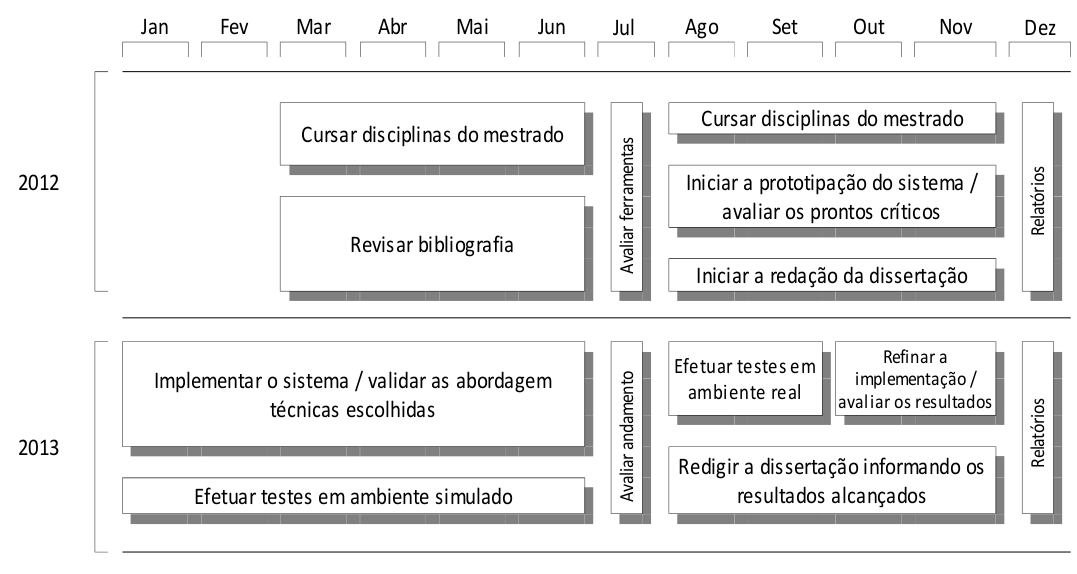
\includegraphics[width=15cm,height=10cm,]{images/chrono.png}
%\centering
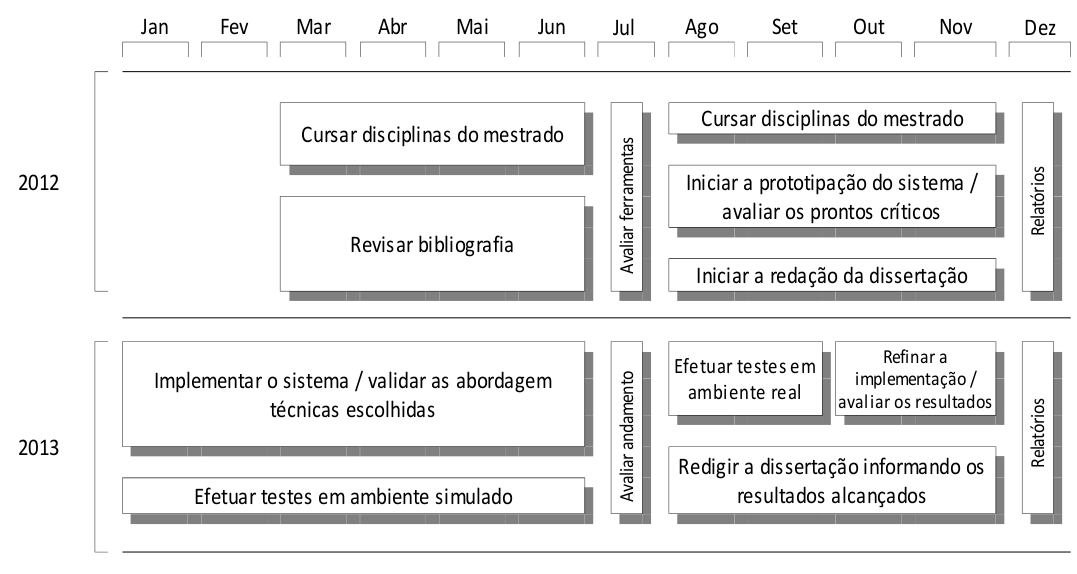
\includegraphics[width=16cm,height=8cm]{images/chrono.png}



\begin{comment}
Sigla	Nome da Disciplina	Início	Término	Carga Horária	Cred.	Freq.	Conc.	Exc.
Situação
SCC5900-1/3	Projeto de Algoritmos	12/03/2012	29/06/2012	180	12	100	A	N Concluída
SSC5858-1/4	Introdução aos Sistemas Evolutivos	12/03/2012	27/04/2012	60	4	85	A	N	Concluída 
SSC5884-1/4	Introdução aos Sistemas Embarcados	12/03/2012	27/04/2012	60	4	100	A	N	Concluída
SSC5887-1/4	Introdução aos Sistemas Robóticos	12/03/2012	27/04/2012	60	4	100	A	N	Concluída
SMA5839-15/2	Preparação Pedagógica	12/03/2012	29/06/2012	60	4	100	A	N	Concluída
SSC5880-2/2	Algoritmos de Estimação para Robótica Móvel	07/05/2012	29/06/2012	90	6	100	A	N	Concluída
SSC5888-2/2	Robôs Móveis Autônomos	07/05/2012	29/06/2012	90	6	100	A	N	Concluída
SCC5878-3/1	Metodologia de Pesquisa Científica em Inteligência Artificial	06/08/2012	07/12/2012	180	12	94	A	N	Concluída
SSC5890-2/2	Algoritmos de Estimação de Distribuição	06/08/2012	05/10/2012	90	6	100	A	N	Concluíd
\end{comment}


--- falar dos testes e melhorias da odometria do carina I

Uma das necessidades básicas para a navegação autônoma é o conhecimento da
localicação do veículo. Para esta localização a odometria do veículo tem papel
importante em informar o deslocamento e pose do veículo durante o seu movimento.
A abordagem para a localização do veículo neste projeto é através do uso do GPS,
que também é possível obter os dados de odometria a partir deste sensor. Um dos
problemas associados ao GPS é a localização mais precisa em pequenos
deslocamentos como manobras de desvio de obstáculos. Já uma odometria baseada em
encoder nas rodas do veículo permitem uma odometria mais precisa nestas
condições, porém diverge rapidamente em maiores distâncias. A abordagem que está
sendo cosiderada é a integração das duas odometrias (pelo encoder e pelo GPS)
através de um filtro extendido de Kalman que estima e atualiza a odometria.

Foram efetuados experimentos com a odometria baseada em encoder na plataforma
CaRINA I que levaram à necessidade de melhorias neste módulo do veículo. Foi
desenvolvido um novo módulo de odometria baseado no encoder da roda e da barra
da direção integrado com os dados da unidade de medida inercial (IMU) que está
sendo utilizada no projeto. O novo módulo também tem ajustes no calculo da
geometria Ackermann levando em consideração as 4 rodas do veículo resultando em
uma melhor estimação da odometria.


Estão sendo realizados experimentos com navegação por GPS baseada em waypoints. 

..Um experimento realizado no âmbito da navegação autônoma 


Foram feitos experimentos de navegação baseado em seguir a força do sinal de
transmissão de rede wi-fi, entre o veículo e uma base fixa. Estes experimentos
resultaram da participação em um artigo 


 No mês de dezembro foi 

 --- falar dos experimentos para o artigo do PSO
--- falar dos experimentos de comunicacao no campus II
--- falar dos experimentos do follow-me
--- falar do setup de simulacao do projeto
--- > 


Exame de Qualificação do Mestrado e Situação Atual no Curso



Etapas resultados:

A primeira etapa consistem em avaliar o sistema em ambiente simulado. A
validação por simulação permite gerar diversas situações desejadas para testar
variados comportamentos sem a necessidade de criá-las no ambiente real, o que
dependendo do cenário pode ser arriscado. A simulação permite maior controle
sobre o ambiente permitindo cenários mais propícios e menos propícios afim de
verificar a robustez do sistema. As análises em ambiente real serão comparadas
com os testes efetuados em simulação permitindo uma avaliação do desempenho,
tanto da qualidade das trajetórias geradas como a capacidade de desvio de
obstáculos.


\section{Contribuições Esperadas}

As principais contribuições acadêmico-científicas esperadas deste trabalho são: 

\begin{enumerate}[i.]

\item adaptação e aperfeiçoamento dos algoritmos para a geração em “tempo real”
de mapas de disparidade, obtendo estes mapas a partir de um par de imagens
capturadas pela câmera estéreo;

\item proposta e desenvolvimento de algoritmos para a obtenção de mapas locais
de navegabilidade com informações espaciais (3D), onde o espaço tridimensional
será dividido em regiões e estas regiões serão identificadas como sendo
navegáveis ou não navegáveis;

\item aperfeiçoamento de técnicas para a navegação baseada no uso de GPS,
bússola e mapas locais de navegabilidade, onde as pesquisas previamente
desenvolvidas para detectar e desviar de obstáculos com o uso de mapas 2D, serão
estendidas a fim de trabalhar com mapa de navegabilidade/ocupação em 3D. Deste
trabalho resultará um sistema com possibilidade de aplicação prática em
importantes tarefas de navegação autônoma, como por exemplo, em sistemas
voltados para aplicações agrícolas e em sistema de combate a incêndio em
florestas, tarefas estas que podem ser perigosas para o ser humano (por exemplo,
exposição prolongada aos produtos químicos de defensivos agrícolas, e
combate/contato direto com fumaça e incêndios).

\end{enumerate}









\section{Resumo}

O objetivo deste trabalho é pesquisar, propor e desenvolver um sistema que
capacite um veículo terrestre a se locomover de modo autônomo em ambientes
externos não estruturados ou pouco estruturados, ou seja, em um campo com
vegetação/plantação e/ou em uma floresta pouco densa (\textit{outdoor} e
\textit{off-road}). O veículo deverá ser capaz de se dirigir até uma localização
pré-determinada (coordenada GPS) escolhendo por meios próprios o caminho a
seguir, ao mesmo tempo em que desvia de obstáculos, percebendo-os de forma
autônoma. O sistema de navegação autônoma irá se basear na aquisição e
processamento de imagens, obtidas a partir de um par de câmeras (câmera
estéreo), constituindo assim um sistema de visão binocular do qual é possível se
obter uma percepção tridimensional do ambiente. Portanto, pretende-se extrair
parâmetros de navegabilidade do ambiente percebido pela câmera estéreo, como
caminhos livres, obstruções e obstáculos, que combinados com as informações de
posição e orientação do veículo e do ponto de destino (baseando-se em
coordenadas de GPS) serão integrados em um sistema robusto de navegação.

Inicialmente serão estudados e trabalhados algoritmos para a criação do mapa de
disparidade a partir do par de imagens obtidas pela câmera estéreo.
A partir do mapa de disparidade, será elaborado um mapa local de navegabilidade
que irá processar e classificar o espaço tridimensional percebido, separando e
representando as regiões navegáveis (seguras) e as regiões não navegáveis
(obstáculos e regiões à evitar) do espaço em frente ao veículo. Este mapa local
será utilizado em conjunto com as informações de posição atual e de destino (GPS
e bússola) a fim de realizar o controle da navegação do veículo. Estão sendo
consideradas duas abordagens principais para o controle local da navegação: a
primeira baseada no uso de Redes Neurais Artificiais, conforme proposto em
trabalhos anteriores desenvolvidos por membros do grupo do LRM e a segunda
baseada em uma adaptação do algoritmo VFH. Nestas abordagens serão consideradas
como parâmetro de entrada as informações tridimensionais do mapa de
navegabilidade. As principais contribuições esperadas deste trabalho são a
adaptação e aperfeiçoamento dos algoritmos para a geração de mapas de disparidade, a
proposta e o desenvolvimento de algoritmos para a obtenção de mapas locais de
navegabilidade com informações espaciais (3D), e por fim o aperfeiçoamento de
técnicas previamente desenvolvidas para detectar e desviar de obstáculos em
mapas 2D, a fim de permitir uma navegação baseada no mapa de navegabilidade 3D.

\section{Objetivo geral}

O objetivo geral deste trabalho é desenvolver um sistema de navegação autônoma baseado
em visão computacional a fim de capacitar um veículo terrestre autônomo a se locomover em
ambientes externos não estruturados, ou seja, em campos com vegetação/plantação e/ou em
florestas pouco densas. O veículo deverá ser capaz de se dirigir até uma localização determinada,
desviando dos obstáculos, percebendo-os de forma autônoma, e escolhendo por meios próprios o
caminho a seguir. O veículo autônomo deverá ter a capacidade de identificar os elementos do terreno
onde irá se deslocar, identificando o chão e os obstáculos, a fim de evitar zonas não transponíveis ou
muito acidentadas. Portanto, o objetivo deste trabalho é desenvolver um sistema de navegação
robusto e seguro voltado à aplicação em veículos autônomos para ambientes externos não
estruturados (ou muito pouco estruturados), baseado no uso de visão computacional realizada
através da captura de imagens estéreo, no uso de mapas de profundidade (mapas de disparidade), e
no uso mapas locais de navegabilidade.

\section{Objetivos Específicos}

Os principais objetivos específicos deste projeto de mestrado, que se apresentam
como um desdobramento do objetivo geral descrito acima, são:

\begin{itemize}

\item Extração de referenciais a partir de um par de câmeras, constituindo um
sistema de visão binocular (estéreo);

\item Propor melhorias nos algoritmos de geração do mapa de disparidade, obtido
a partir das imagens estéreo;

\item Gerar um mapa de navegabilidade local a partir de informações visuais;
%,
%que possa ser adaptado a algoritmos de planejamento e controle de navegação
%autônoma;

\item Desenvolver um mecanismo de navegação autônoma, baseado nas informações de
GPS, Bússola e do Sistema de Visão, capaz de desviar de obstáculos e dirigir o
veículo até um destino determinado de forma robusta e eficiente;

\item Fazer uso dos conhecimentos prévios de trabalhos desenvolvidos no
laboratório e contribuir para a consolidação de tecnologias capazes de atribuir
navegabilidade autônoma a veículos de diversas naturezas para fins práticos;

\item Aplicação e avaliação do sistema de navegação autônoma em um veículo real
em ambiente externo não estruturado.

\end{itemize}


\section{Atividades Realizadas}



\section{Resultados Parciais}

\begin{frame}
\frametitle{Resultados parciais}
\framesubtitle{Arquitetura do sistema}
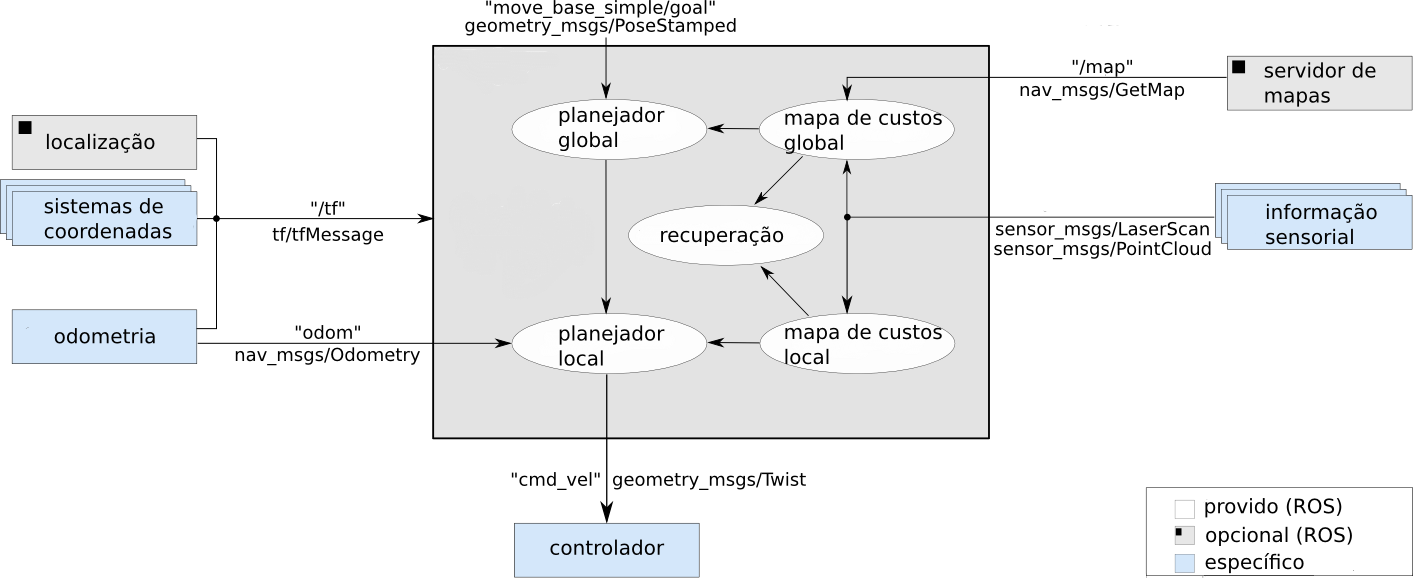
\includegraphics[width=10cm,height=7cm,]{../img/overview_tf_pt.png}
\end{frame}

\begin{frame}
\frametitle{Resultados parciais}
\framesubtitle{Modelagem do veículo}
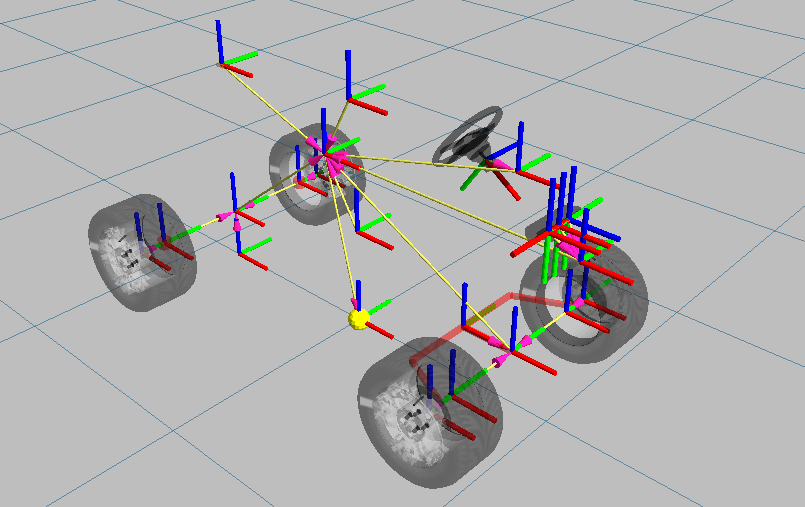
\includegraphics[width=10cm,height=7cm,]{../img/carina_tf_side_wheels_transp.png}
\end{frame}

\begin{frame}
\frametitle{Resultados parciais}
\framesubtitle{Modelagem do veículo}
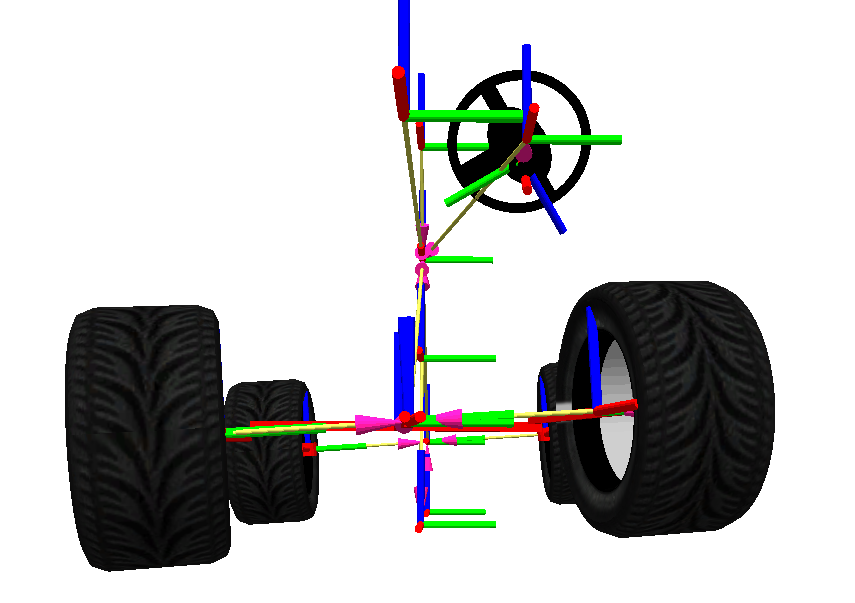
\includegraphics[width=10cm,height=7cm,]{../img/carina_rviz_uneven_susp.png}
\end{frame}


\begin{frame}
\frametitle{Resultados parciais}
\framesubtitle{Odometria e Localização por GPS}
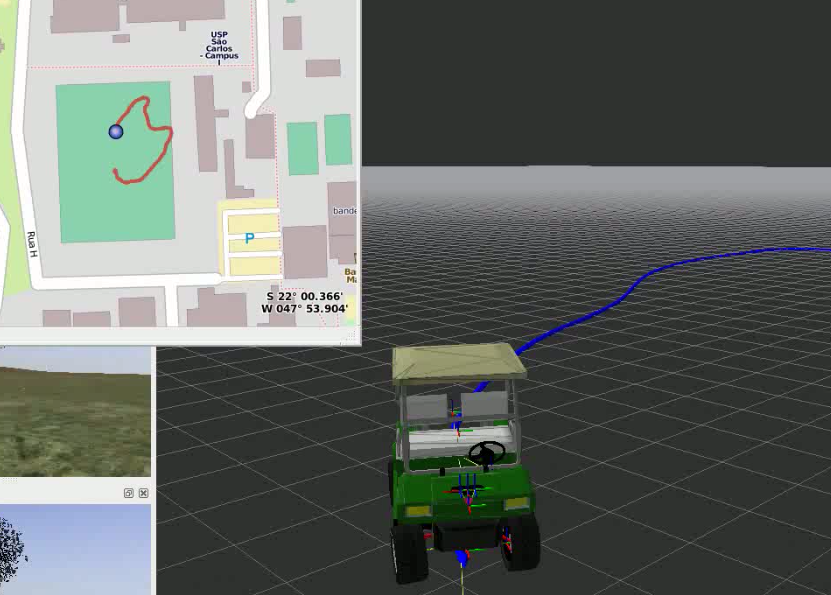
\includegraphics[width=10cm,height=7cm,]{../img/arq_odogps.png}
\end{frame}


\begin{frame}
\frametitle{Resultados parciais}
\framesubtitle{Imagem - Câmera Estéreo}
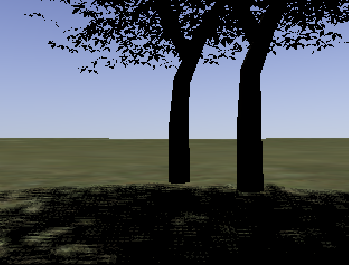
\includegraphics[width=10cm,height=7cm,]{../img/arq_image.png}
\end{frame}

\begin{frame}
\frametitle{Resultados parciais}
\framesubtitle{Cálculo da disparidade}
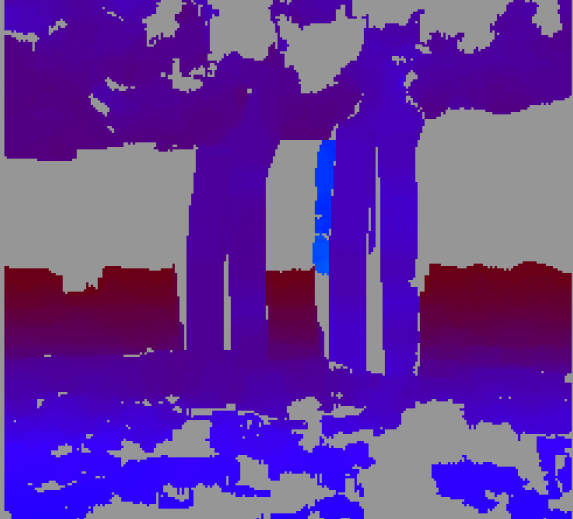
\includegraphics[width=10cm,height=7cm,]{../img/arq_disp.png}
\end{frame}

nesta etapa é efetuado o cálculo da disparidade entre os pixeis das imagens
relacionadas. A principal dificuldade deste cálculo é fazer a correspondência
entre cada pixel, isto é, verificar qual pixel em cada imagem
corresponde ao mesmo ponto na cena. Algoritmos que fazem esta busca são de forma
geral classificados como busca local, semi-global e global, onde o custo
computacional tende a ser maior nos métodos globais. Foram testados dois
métodos, um local e um semi-global. O método local Block Matching tem se
demonstrado suficiente para gerar a disparidade com um custo computacional que
permite aplicação em tempo real. 

\begin{frame}
\frametitle{Resultados parciais}
\framesubtitle{Nuvem de pontos}
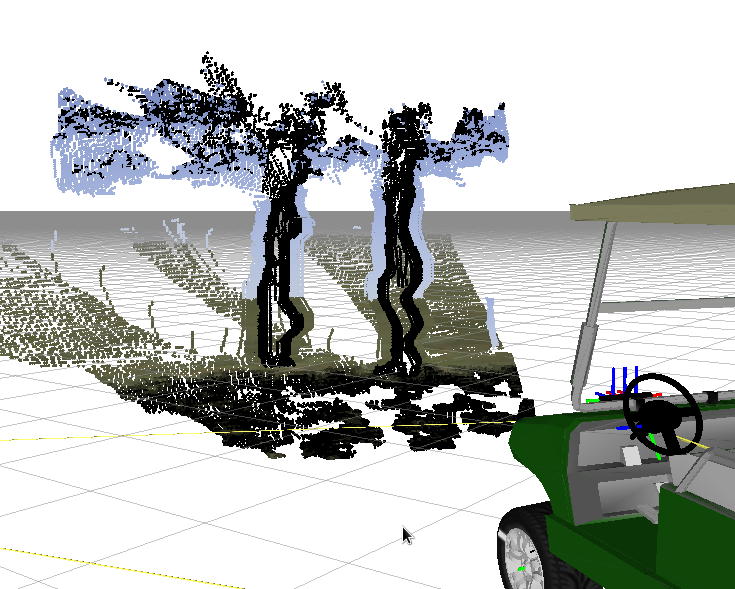
\includegraphics[width=10cm,height=7cm,]{../img/arq_cloud.png}
\end{frame}

Uma nuvem de pontos é construida a partir das disparidades calculadas no passo
anterior. Enquanto a disparidade é apenas uma distancia relativa em pixeis de
cada ponto correlacionado, a nuvem de pontos fornece a informação tridimensional
métrica da posição do ponto no espaço. Porém, a nuvem de pontos é uma
representação não estruturada dos dados da cena, sendo então necessário uma
forma de armazenar e fazer buscas nestes dados de forma estruturada.

\begin{frame}
\frametitle{Resultados parciais}
\framesubtitle{Octomap - Discretização/Agrupamento}
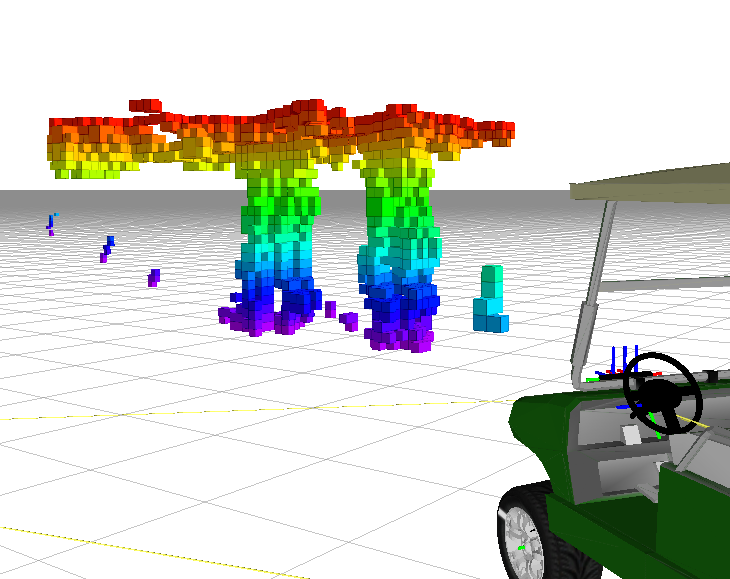
\includegraphics[width=10cm,height=7cm,]{../img/arq_octomap.png}
\end{frame}

A representação da nuvem de pontos em um Octomap permite uma noção agrupada
dos dados assim como uma relação entre pontos vizinhos em uma estrutura em
forma de árvore. Desta forma já é possível analisar os dados de forma
estruturada e o armazenamento da informação também se torna mais reduzido devido
ao agrupamento feito pela octree discretizando o espaço em volumes cúbicos de
tamanhos variáveis 

%(maiores onde há menor volume de pixeis, menores onde há maior concentração de
% pixies).

\begin{frame}
\frametitle{Resultados parciais}
\framesubtitle{Mapa de Ocupação / Navegabilidade}
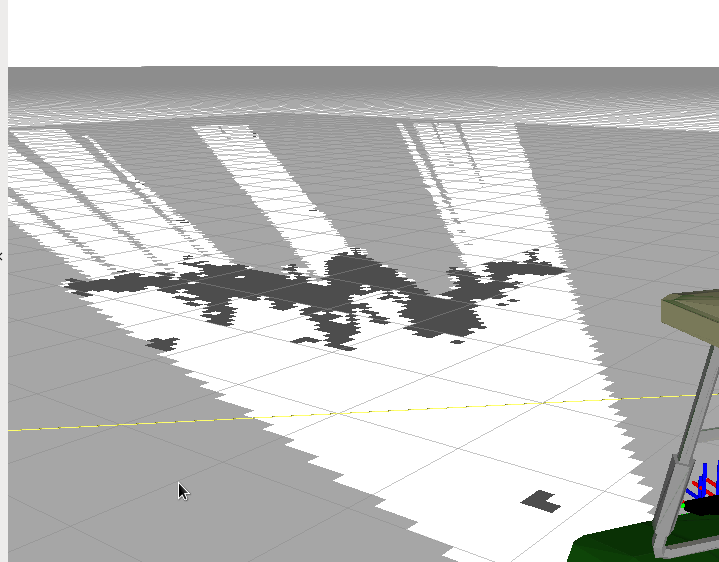
\includegraphics[width=10cm,height=7cm,]{../img/arq_mapa.png}
\end{frame}

A partir dos dados já agrupados em uma octree é possível analisar de forma
estruturada a ocupação do espaço, assim, gerando um mapa de navegabilidade
baseada na informação de ocupação ou não do espaço

% e também da concentração de pixeis em uma determinada área que 


As próximas etapas do projeto consistem em criar o mapa de navegabilidade de
forma que a informação tridimensional captada pela câmera estéreo possa ser
agregada ao planejamento de navegação autônoma do veículo. 

Os experimentos em simulação serão validados no ambiente real em um cenário
limitado porém com as características definidas no projeto, ou seja, um cenário
externo não estruturado.




Experimento: Geração de Waypoints intermediários baseado em um mapa topográfico
georeferenciado.

Dado um mapa topográfico georeferenciado, a elevação do terreno é convertida em
custos a partir do cálculo da derivada da superfície indicando o quão íngrime é
o deslocamento de um ponto ao outro. Determinadas altitudes (altura e
profundidade) também podem ser atribuidos custos fixos elevados para inibir a
geração de um caminho nestes pontos. O algoritmo T-RRT é executado tendo como
entrada este mapa de custos, o T-RRT produz então um caminho de menor custo
indicando os pontos intermediários. Como o mapa é georeferenciados esses pontos
do caminho podem ser utilizados como waypoints de GPS intermediários para a
navegação entre pontos origem/destino distantes de forma a produzir uma
tragetória idealmente de menor dificuldade de navegação.

Esta abordagem foi testada com o propósito de avaliar o algoritmo T-RRT e
verificar a sua capacidade de gerar uma tragetória baseada em waypoints para a
navegação em áreas extensas. Pelos testes a técnica se demonstrou
satisfatória porém ainda não foi feito nenhum experimento de navegação a partir
destes resultados. 


Experimento: Navegação baseada na atração pela potência do sinal de rede wi-fi.

No contexto deste projeto, este experimento teve como pricipal propósito a
familiarização com o ambiente de simulação e as ferramentas 



Experimento: Navegação em desvio de obstáculos baseada em RNA

Este experimento basicamente foi a replicação de uma aplicação de Rede Neural
Artficial (RNA) para a navegação e desvio de obstáculos desenvolvida por um
colega do laboratório. No experimento original foi modelado um veículo com
características específicas, seguindo o modelo Ackermann. Originalmente foi 
desenvolvido um simulador próprio e o treinamento de uma RNA foi efetuado em um
cenário sintético de exemplo contendo obstáculos espaçados simulando árvores. A
replicação do experimento constituiu em passar toda a modelagem para o ambiente
ROS e o simulador Gazebo já com o modelo virtual do veículo CaRINA I de acordo
com as características deste veículo. O novo cenário foi baseado no cenário
original e a rede neural utilizada foi a mesma, ou seja, não houve novo
treinamento, apenas foi aplicada ao novo cenário e o novo veículo simulando as
mesmas condições sensorias baseada em laser. Nos testes, a rede neural conseguiu
navegar e desviar dos obstáculos de forma semelhante ao experimento original
verificando a viabilidade do uso desta técnica.




\subsubsection{Navegação}

Para a navegação autônoma deliberativa/reativa é necessário o planejamento da
trajetória e o controle do veículo em relação a aceleração e esterçamento.
Conforme definido na arquitetura apresentada, há um planjemento global, que
define o comportamento deliberativo do veículo, onde uma trajetória é planejada
levando em consideração o espaço navegável conhecido pelo veículo (através do
mapa). Para este planejamento global está sendo considerada a abordagem de
geração de trajetórias por amostras utilizando a técnica SBPL. O planejamento
local basicamente são ações reativas tomadas pelo veículo em relação aos
obstáculos próximos e condições dinâmicas do ambiente. A utilização da técnica
VFH e mesmo o uso de RNA já foram testadas em trabalhos anteriores se
demonstrando eficazes em aplicações reais para o controle e navegação do veículo
de modo reativo. Todas estas abordagens estão sendo consideradas neste projeto
por já terem sido validadas em trabalhos anteriores desenvolvidos no LRM, porém
ainda poderão ser consideradas outras abordagens para estes componentes da
arquiterura caso se adaptem melhor aos mapas que serão gerados. Porém estes
aspectos estão mais associados ao funcionamento completo do sistema e não ao
principal foco da pesquisa que está voltado à geração de mapas de navegabilidade
a partir de informações provenientes do aplicação de visão estéreo.




\end{document}
